%%%%%%%%%%%%%%%%%%%%%%%%%%%%%%%%%%%%%%%%%%%%%%%%%%%%%%%%%%%%%%%%%%%%%%%%%%%%%%
\section{Simulation of the $\pi+ \to e^+ \nu $ signal }

The \piplusenu\ signal is simulated using the standard Mu2e multi-stage simulation scheme.
\begin{itemize}
\item
  stage 1: simulation of the proton interactions in the PT and tracing the pions 
  till the DS entrance. The pion decays are turned off, the TS3 collimator is rotated
  by 180 degrees. Statistics: $2.5 \times 10^8$ POT.
\item
  stage 2: tracing the pions till they stop in the degrader or in the ST. A Ti degrader is placed
  at the DS entrance. The degrader thickness is varied in the range 2-5 mm with a step of 1 mm.
\item
  stage 3: simulation of the $\pi^+ \to e^+ \nu$ decays in the detector 
\item
  stage 4: digitization. The digitization start moved down to 100 ns ;
\item
  stage 5: reconstruction and ntupling. The earliest time used by the reconstruction algorithms
  is moved down to 100 ns ;
\item
  the constant, representing the time offset between the proton bunch arrival
  to the stopping target and the DAQ data request, is set to zero.
\end{itemize}

Stage 1 is common for all datasets. Starting from stage 2, datasets corresponding
to different degrader thicknesses required separate generation.

\begin{table}[H]
\begin{tabularx}{1.0\textwidth} {|X|c|c|c|c|c|}  %
% \begin{tabular}{1.0\textwidth} {|l|l|}  %
  \hline
  Dataset             & degrader thickness & N(ST)       & N(DEG stops) & sum W ST  & sum W(deg)   \\
                      & (mm)               &             &              &           &              \\
  \hline                                                                                          
  bpip0b0             &  no degrader       &   312616    &     0        &   105.7   &              \\
  \hline                                                                                          
  bpip2b0             &     2              &   84785     &   448131     &   276.6   &   454.7      \\
  \hline                                                                                          
  bpip3b0             &     3              &   50340     &   532767     &  272.7    &   977        \\
  \hline                                                                                        
  bpip4b0             &     4              &   31681     &   583855     &  236      &  1537        \\
  \hline                                                                                          
  bpip5b0             &     5              &   17225     &   617324     &  158.8    &   2070       \\
  \hline
\end{tabularx}
\end{table}

Distributions of the pion stop time for pion stopped in the ST and the degrader are shown
in Figure~\ref{fig:pion_stop_time}. A probability for a pion produced at the PT to reach the
the stopping target and stop there could 

\begin{figure}[H]
  \begin{tikzpicture}
    \node[anchor=south west,inner sep=0] at (0,0.) {
      % \node[shift={(0 cm,0.cm)},inner sep=0,rotate={90}] at (0,0) {}
      \makebox[\textwidth][c] {
        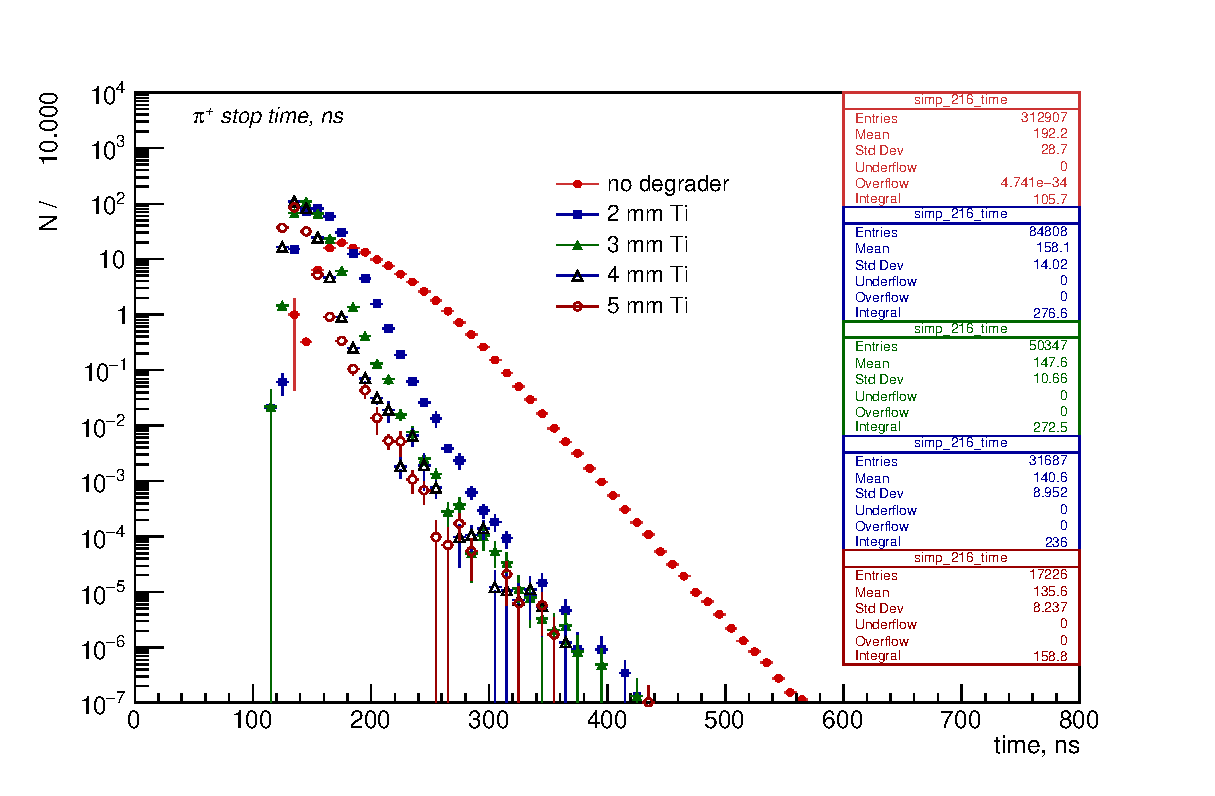
\includegraphics[width=0.55\textwidth]{pdf/figure_02002}
        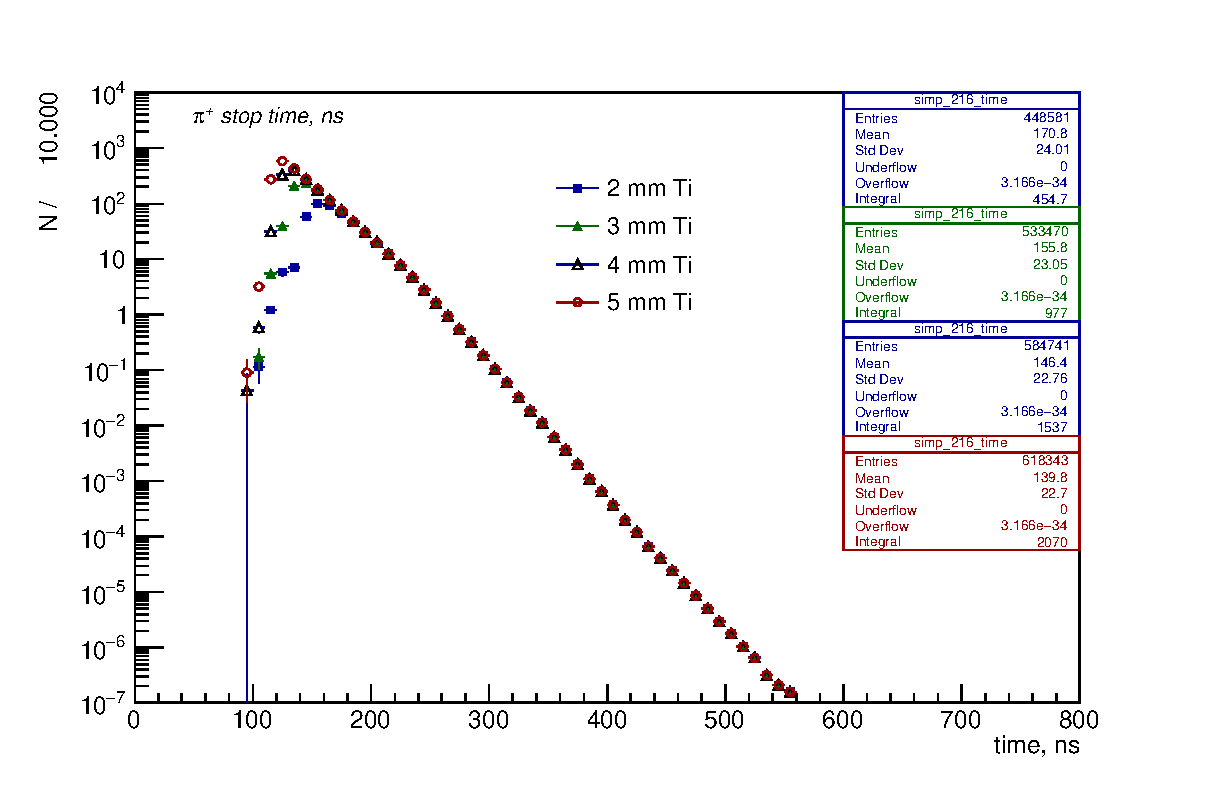
\includegraphics[width=0.55\textwidth]{pdf/figure_02402}
      }
    };
    % \node [text width=8cm, scale=1.0] at (14.5,0.5) {$\mu_B$, expected background mean};
    % \node [text width=8cm, scale=1.0, rotate={90}] at (1.5,7.5) { $S_{D}$, ``discovery'' signal strength  };
  \end{tikzpicture}
  \caption{
    \label{fig:pion_stop_time}
    Distributions of pi stop time for pions stopping in the ST (left) and degrader (right).
    The events are weighted with the pion survival probability.
    The integrals are the sums of individual event weights.
  }
\end{figure}

It is interesting to note that as the degrader thickness increases, the probability for a positive pion
to reach the stopping target and stop there first increases to reach $\sim 10^{-6}$, and after 3-4mm
starts falling down.  The probability for a pion to stop in the degrader continues to increase,
however the increase is due to the stops of faster and faster pions, so additional events accumulate
only at early times, below 200 ns.

The Z distribution of the $\pi^+$ stops, plotted via its ST foil number  proxy, is shown
in Figure~\ref{fig:pion_stop_foil}. The yield of stopped pions is maximize for the degrader
thickness of about 2-3 mm Ti.

\begin{figure}[H]
  \begin{tikzpicture}
    \node[anchor=south west,inner sep=0] at (0,0.) {
      % \node[shift={(0 cm,0.cm)},inner sep=0,rotate={90}] at (0,0) {}
      \makebox[\textwidth][c] {
        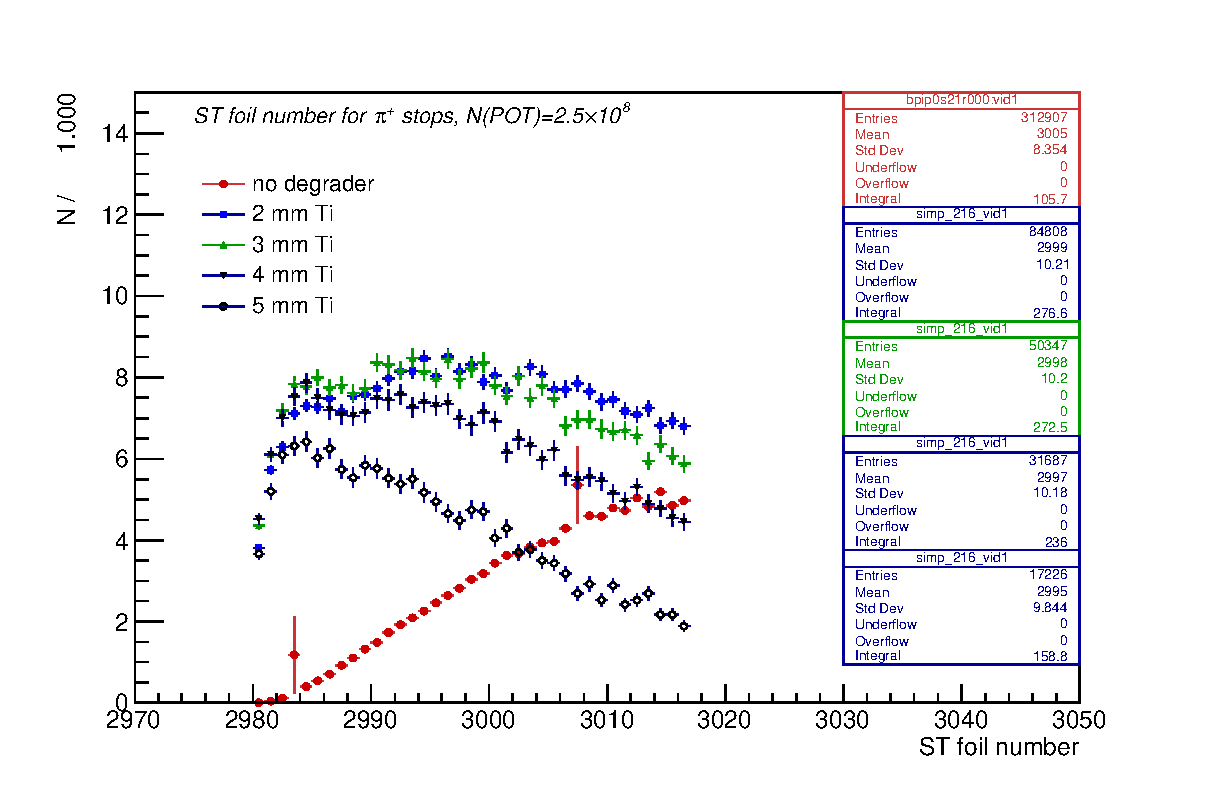
\includegraphics[width=0.90\textwidth]{pdf/figure_00009}
      }
    };
    % \node [text width=8cm, scale=1.0] at (14.5,0.5) {$\mu_B$, expected background mean};
    % \node [text width=8cm, scale=1.0, rotate={90}] at (1.5,7.5) { $S_{D}$, ``discovery'' signal strength  };
  \end{tikzpicture}
  \caption{
    \label{fig:pion_stop_foil}
    Distributions of the pion stop Z (ST foil number) for different thicknesses
  }
\end{figure}

%%%%%%%%%%%%%%%%%%%%%%%%%%%%%%%%%%%%%%%%%%%%%%%%%%%%%%%%%%%%%%%%%%%%%%%%%%%%%%
\newpage
\subsection {{\red Validation: turning off pion decays  Sridhar}}

Weighting events with the pion lifetime - validation plot here

\begin{figure}[H]
  \begin{tikzpicture}
    \node[anchor=south west,inner sep=0] at (0,0.) {
      % \node[shift={(0 cm,0.cm)},inner sep=0,rotate={90}] at (0,0) {}
      \makebox[\textwidth][c] {
        \includegraphics[width=0.8\textwidth]{pdf/figure_00105}
      }
    };
    \node [text width=8cm, scale=1.0] at (14.5,0.5) {$\mu_B$, expected background mean};
    \node [text width=8cm, scale=1.0, rotate={90}] at (1.5,7.5) { $S_{D}$, ``discovery'' signal strength  };
  \end{tikzpicture}
  \caption{
    \label{fig:pion_lifetime}
  }
\end{figure}

To increase statistics, the pion beam simulation had the charged pion decays turned off.
The survival probability of stopped $\pi^+$'s was stored and used in the analysis
as the event weight. For validation, start momenta of stopped $\pi^+$'s for two datasets, one with pion decay turned off and other with turned on, have been compared in Figure~\ref{fig:pion_lifetime}. The intergrals validating approximately similar gains. 

